% !TEX encoding = UTF-8 Unicode

%
% Exemple de rapport
% par Pierre Tremblay, Universite Laval
% modifié par Christian Gagne, Universite Laval
% modifié par Francis Valois, Université Laval
% 31/01/2011 - version 1.4
%

%
% Modele d'organisation d'un projet LaTeX 
% rapport/      dossier racine et fichier principal
% rapport/fig   fichiers des figures
% rapport/tex   autres fichiers .tex
%

% ** Preambule **
%
% Ajouter les options au besoin :
%    - "ULlof" pour inclure la liste des figures, requis si "\begin{figure}" utilise
%    - "ULlot" pour inclure la liste des tableaux, requis si "\begin{table}" utilise
%
\documentclass[12pt,ULlof,ULlot]{ULrapport}

% Chargement des packages supplementaires (si absent de la classe)
\usepackage[utf8]{inputenc}
\usepackage[T1]{fontenc}
\usepackage[autolanguage]{numprint}
\usepackage{icomma}
\usepackage{subfigure}
\usepackage{graphicx}
\usepackage[absolute]{textpos}
\usepackage[final]{pdfpages}
\def\dbar{{\mathchar'26\mkern-12mu d}} 
%\usepackage[options]{nom_du_package}

% Definition d'une commande pour presenter des cellules multilignes dans un tableau
\newcommand{\cellulemultiligne}[1]{\begin{tabular}{@{}c@{}}#1\end{tabular}}


% Definition de colonnes en mode paragraphe avec alignement ajustable
% Cette definition requiert le chargement du package "array"
%    - alignement horizontal, parametre #1 : - \raggedright (aligne a gauche)
%                                            - \centering (centre)
%                                            - \raggedleft (aligne a droite)
%    - alignement vertical, parametre #2 : - p (aligne en haut)
%                                          - m (centre)
%                                          - b (aligne en bas)
%    - largeur, parametre #3 : longueur
\newcolumntype{Z}[3]{>{#1\hspace{0pt}\arraybackslash}#2{#3}}

% Definitions des parametres de la page titre
\TitreProjet{Rapport de laboratoire 0}                         % Titre du projet
\TitreRapport{Systèmes de communications}       % Titre du rapport
\Destinataire{M. Jean-Yves Chouinard}         % Nom(s) du destinataire
\TableauMembres{%                                     % Tableau des membres de l'equipe
   910\,055\,897  & Daniel Thibodeau \\\hline
   910\,097\,879  & Francis Valois \\\hline        % matricule & nom & \\\hline
           % matricule & nom & \\\hline     % matricule & nom & \\\hline
}
\DateRemise{21 septembre 2012}                           % Date de remis


% Corps du document

\begin{document}

%   Chapitres
%%!TEX root = ../rapport.tex
%!TEX encoding = UTF-8 Unicode

% Chapitres "Introduction"

% modifié par Francis Valois, Université Laval
% 31/01/2011 - version 1.0 - Création du document

\chapter{Introduction}
\label{s:introduction}

%!TEX root = ../rapport.tex
%!TEX encoding = UTF-8 Unicode

\chapter{Préparation}
\section*{Numéro 1}
\subsection*{a)}

Sachant que le signal MF possède une équation de la forme suivant :

\begin{equation}
	S_{MF} = A\cos(2\pi f_c t + 2\pi k_f \int m(t)dt)
\end{equation}

Et que le message envoyé est le suivant :
\begin{equation}
	m(t) = B \cos(2\pi f_m t)
\end{equation}

Alors l'intégrale du message est l'équation suivante :
\begin{equation}
	m(t)_i = \frac{B}{2\pi f_m}\sin(2\pi f_m t)
\end{equation}

Et le signal envoyé est le suivant :

\begin{equation}
	S_{MF} = A\cos(2\pi f_c t + \frac{B k_f}{f_m}\sin(2\pi f_m t))
\end{equation}


\begin{equation}
	S_{MF} = 10 \cos(2\pi 10^6 t + \frac{5 }{}\sin(2000\pi  t))
\end{equation}


\subsection*{b)}

L'indice de modulation peut être calculé a l'aide de l'équation suivante :

\begin{equation}
	\beta = \frac{\Delta}{f_m} = \frac{K_f max\{m(t)\}}{2\pi f_m}
\end{equation}

Comme le signal m(t) est un cosinus, son amplitude maximale est B

\begin{equation}
	\beta = \frac{5000}{2\pi 1000} = 0.7959
\end{equation}

\subsection*{c)}
La largeur de bande effective est donnée par l'équation suivante :

\begin{equation}
	LB \approx 2(f_m + \Delta f_c)= 2f_m(1+\beta)
\end{equation}

\begin{equation}
	LB \approx  2000(1+0.7959) = 3591.8
\end{equation}


\subsection*{d)}
Selon les tables de Bessel, pour un signal avec un $\beta$ de 0.7959, le signal va posséder un n de 3. Ainsi, la bande passante va être de $3f_m$, soit de 6 kHz.

\subsection*{e)}

Comme le spectre d'un signal FM est donné par l'équation suivante :

\begin{equation}
	e(t) = A \sum^\infty_{n=-\infty} J_n(\beta)\cos(2\pi(f_c+nf_m)t)
\end{equation}

et que pour un $\beta$ de 0.7959, nous avons les 4 valeurs suivantes de $J_n(\beta)$ : 0.85, 0.365, 0.074 et 0.0099. Alors nous aurons 7 raies spectrales comme le montre la figure \ref{schema1}.

\begin{figure}[htb]
\begin{center}
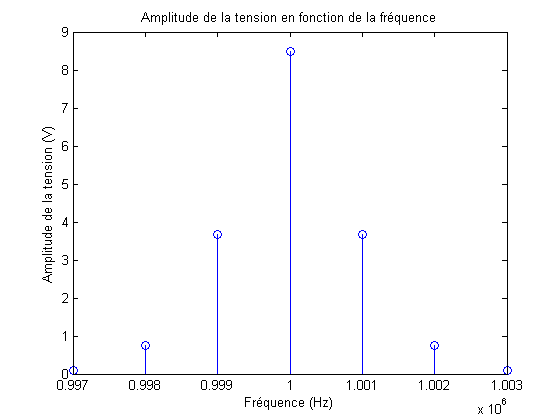
\includegraphics[scale=0.7]{no1e.png}
\caption{Figure représentant le spectre du signal FM demandé}
\label{schema1}
\end{center}
\end{figure}

\section*{Numéro 2}
La figure \ref{schema2} représente l'émetteur à bande large superhétérodyne.

\begin{figure}[htb]
\begin{center}
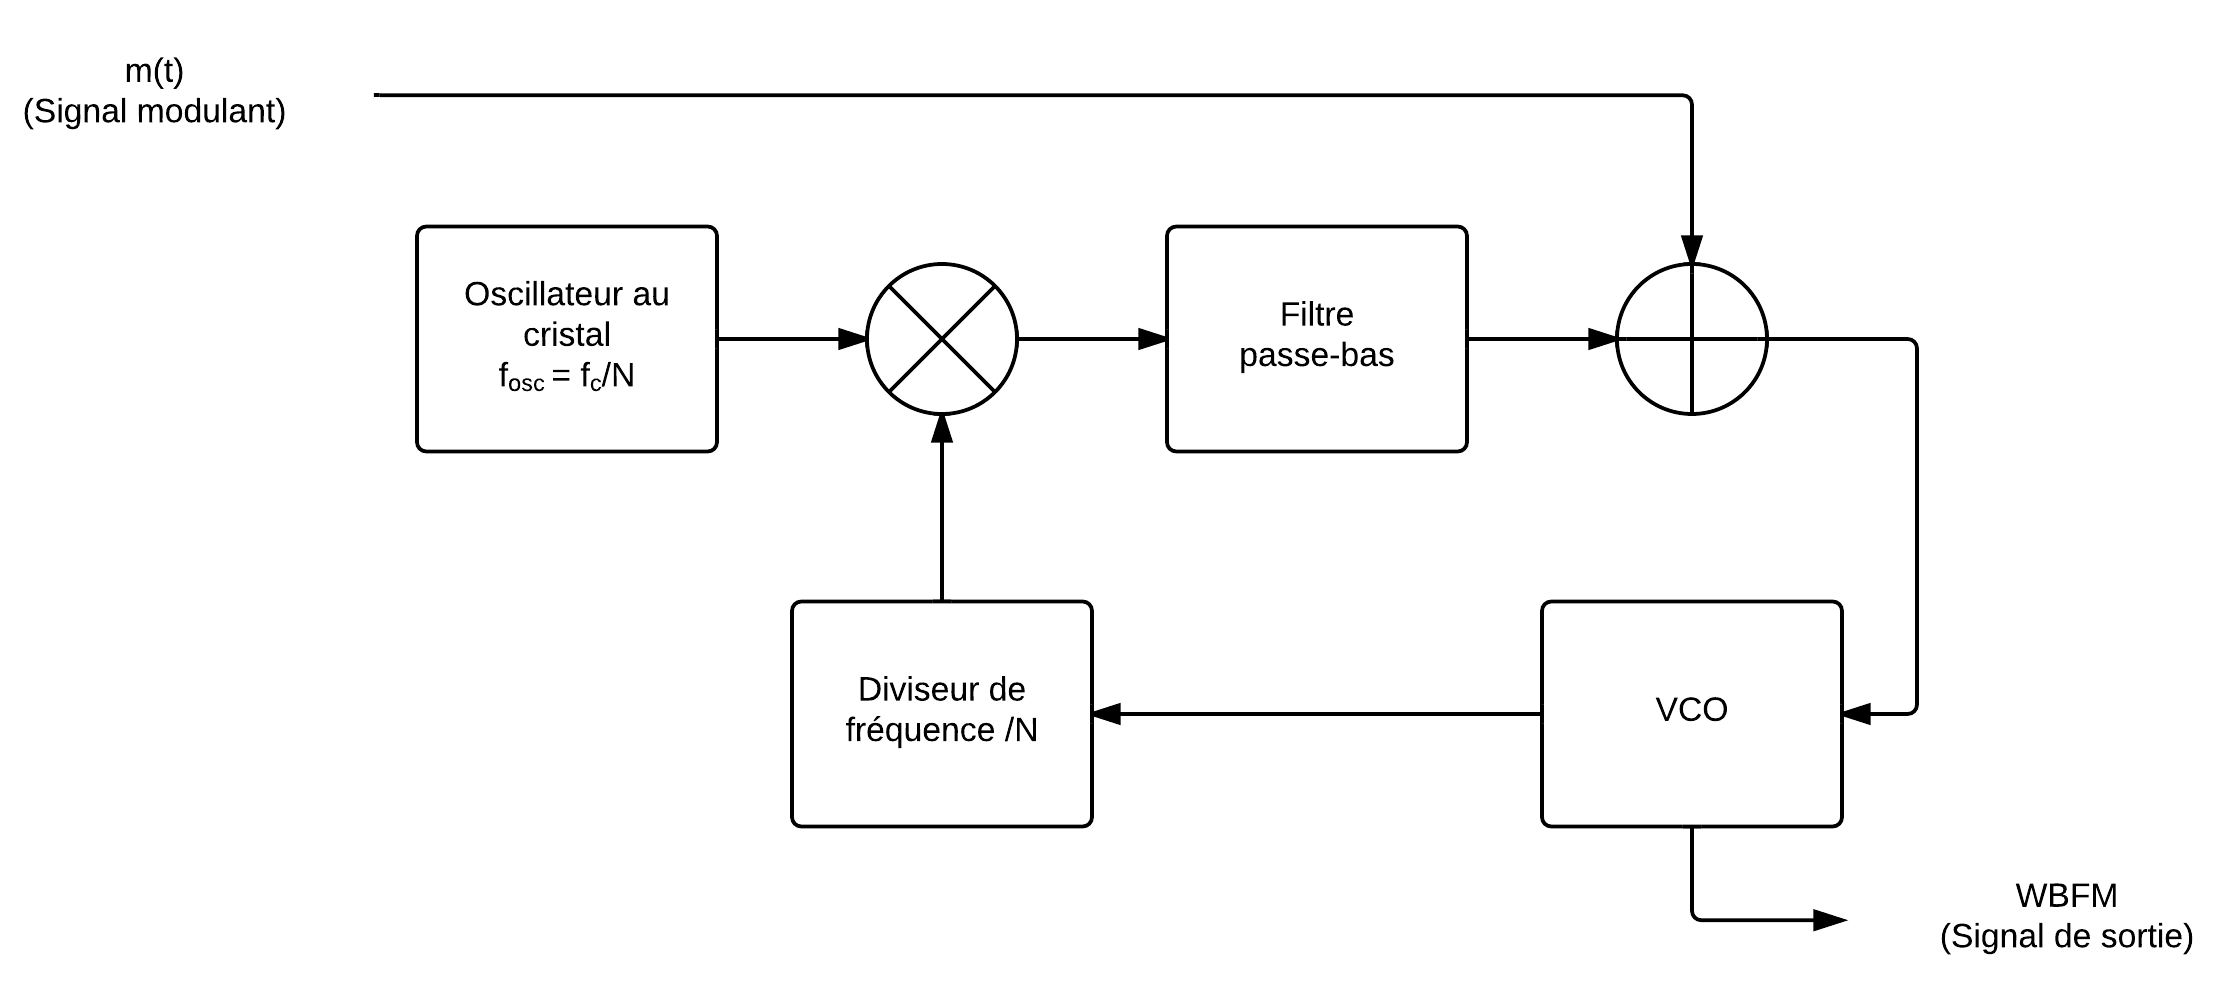
\includegraphics[scale=0.8]{Q2.png}
\caption{Figure représentant l'émetteur à bande large superhétérodyne}
\label{schema2}
\end{center}
\end{figure}

%%!TEX root = ../rapport.tex
%!TEX encoding = UTF-8 Unicode
\chapter{Expérimentation, Analyse, Résultat}


%%!TEX encoding = UTF-8 Unicode
%!TEX root = ../rapport.tex
% Chapitres "Conclusion"

% modifié par Francis Valois, Université Laval
% 31/01/2011 - version 1.0 - Création du document

\chapter{Conclusion}
\label{s:conclusion}

Au cours de ce septième laboratoire, nous nous sommes familiarisé avec l'implantation pratique d'un oscillateur triangulaire pouvant être employé afin de moduler un signal quelconque. Par ailleurs, nous nous sommes aussi familiarisé avec l'implantation d'un comparateur à hystérésis capable d'effectuer ladite modulation en procurant une protection additionnelle contre le buit. Aussi, nous avons su implanté de manière pratique un filtre Butterworth d'ordre 2 ayant pour fonction d'effectuer la démodulation du signal. De par la précision la similitude entre l'onde de sortie et l'onde d'entrée, nous avons pu constater l'efficacité de notre montage et les qualités de la réponse en fréquence du filtre Butterworth. Il est intéressant de noter le déphasage des signaux de sortie, déphasage tout de même significatif, qui provient de la fonction de filtrage qui induit un déphasage non nul dans sa fonction de transfert.

\appendix
%%!TEX root = ../rapport.tex
%!TEX encoding = UTF-8 Unicode
% Chapitres "Annexes"

% modifié par Francis Valois, Université Laval
% 31/01/2011 - version 1.0 - Création du document
\chapter{Annexes}
\label{s:annexes}




\end{document}
% Fin du document

